% Copyright 2021 Politecnico di Milano, Italy. NC-BY

\documentclass{Configuration_Files/PoliMi3i_thesis}

%------------------------------------------------------------------------------
%	REQUIRED PACKAGES AND  CONFIGURATIONS
%------------------------------------------------------------------------------

% CONFIGURATIONS
\usepackage{parskip} % For paragraph layout
\usepackage{setspace} % For using single or double spacing
\usepackage{emptypage} % To insert empty pages
\usepackage{multicol} % To write in multiple columns (executive summary)
\setlength\columnsep{15pt} % Column separation in executive summary
\setlength\parindent{0pt} % Indentation
\raggedbottom  

% PACKAGES FOR TITLES
\usepackage{titlesec}
% \titlespacing{\section}{left spacing}{before spacing}{after spacing}
\titlespacing{\section}{0pt}{3.3ex}{2ex}
\titlespacing{\subsection}{0pt}{3.3ex}{1.65ex}
\titlespacing{\subsubsection}{0pt}{3.3ex}{1ex}
\usepackage{color}

% PACKAGES FOR LANGUAGE AND FONT
\usepackage[english]{babel} % The document is in English  
\usepackage[utf8]{inputenc} % UTF8 encoding
\usepackage[T1]{fontenc} % Font encoding
\usepackage[11pt]{moresize} % Big fonts

% PACKAGES FOR IMAGES
\usepackage{adjustbox}
\usepackage{graphicx}
\usepackage{transparent} % Enables transparent images
\usepackage{eso-pic} % For the background picture on the title page
\usepackage{subfig} % Numbered and caption subfigures using \subfloat.
\usepackage{tikz} % A package for high-quality hand-made figures.
\usetikzlibrary{}
\graphicspath{{./Images/}} % Directory of the images
\usepackage{caption} % Coloured captions
\usepackage{xcolor} % Coloured captions
\usepackage{amsthm,thmtools,xcolor} % Coloured "Theorem"
\usepackage{float}

% STANDARD MATH PACKAGES
\usepackage{amsmath}
\usepackage{amsthm}
\usepackage{amssymb}
\usepackage{amsfonts}
\usepackage{bm}
\usepackage[overload]{empheq} % For braced-style systems of equations.
\usepackage{fix-cm} % To override original LaTeX restrictions on sizes

% PACKAGES FOR TABLES
\usepackage{tabularx}
\usepackage{longtable} % Tables that can span several pages
\usepackage{colortbl}

% PACKAGES FOR ALGORITHMS (PSEUDO-CODE)
\usepackage{algorithm}
\usepackage{algorithmic}

% PACKAGES FOR REFERENCES & BIBLIOGRAPHY
\usepackage[colorlinks=true,linkcolor=black,anchorcolor=black,citecolor=black,filecolor=black,menucolor=black,runcolor=black,urlcolor=black]{hyperref} % Adds clickable links at references
\usepackage{cleveref}
\usepackage[square, numbers, sort&compress]{natbib} % Square brackets, citing references with numbers, citations sorted by appearance in the text and compressed
\bibliographystyle{abbrvnat}

% OTHER PACKAGES
\usepackage{pdfpages} % To include a pdf file
\usepackage{afterpage}
\usepackage{lipsum} % DUMMY PACKAGE
\usepackage{fancyhdr} % For the headers
\fancyhf{}

\usepackage{listings}
\usepackage{xcolor}

\definecolor{codegray}{rgb}{0.5,0.5,0.5}
\definecolor{codepurple}{rgb}{0.58,0,0.82}
\definecolor{backcolour}{rgb}{0.95,0.95,0.95}

\lstdefinestyle{pythonstyle}{
    backgroundcolor=\color{backcolour},
    commentstyle=\color{codegray},
    keywordstyle=\color{blue},
    numberstyle=\tiny\color{codegray},
    stringstyle=\color{codepurple},
    basicstyle=\ttfamily\footnotesize,
    breaklines=true,
    captionpos=b,
    numbers=left,
    numbersep=5pt,
    showspaces=false,
    showstringspaces=false,
    tabsize=4
}
\lstset{style=pythonstyle}

% Input of configuration file.
% Define blue color typical of polimi
\definecolor{bluepoli}{cmyk}{0.4,0.1,0,0.4}

% Custom theorem environments
\declaretheoremstyle[
  headfont=\color{bluepoli}\normalfont\bfseries,
  bodyfont=\color{black}\normalfont\itshape,
]{colored}

% Set-up caption colors
\captionsetup[figure]{labelfont={color=bluepoli}} % Set colour of the captions
\captionsetup[table]{labelfont={color=bluepoli}} % Set colour of the captions
\captionsetup[algorithm]{labelfont={color=bluepoli}} % Set colour of the captions

\theoremstyle{colored}
\newtheorem{theorem}{Theorem}[chapter]
\newtheorem{proposition}{Proposition}[chapter]

% Enhances the features of the standard "table" and "tabular" environments.
\newcommand\T{\rule{0pt}{2.6ex}}
\newcommand\B{\rule[-1.2ex]{0pt}{0pt}}

% Pseudo-code algorithm descriptions.
\newcounter{algsubstate}
\renewcommand{\thealgsubstate}{\alph{algsubstate}}
\newenvironment{algsubstates}
  {\setcounter{algsubstate}{0}%
   \renewcommand{\STATE}{%
     \stepcounter{algsubstate}%
     \Statex {\small\thealgsubstate:}\space}}
  {}

% New font size
\newcommand\numfontsize{\@setfontsize\Huge{200}{60}}

% Title format: chapter
\titleformat{\chapter}[hang]{
\fontsize{30}{20}\selectfont\bfseries\filright}{\textcolor{bluepoli} \thechapter\hsp\hspace{2mm}\textcolor{bluepoli}{|   }\hsp}{0pt}{\huge\bfseries \textcolor{bluepoli}
}

% Title format: section
\titleformat{\section}
{\color{bluepoli}\normalfont\Large\bfseries}
{\color{bluepoli}\thesection.}{1em}{}

% Title format: subsection
\titleformat{\subsection}
{\color{bluepoli}\normalfont\large\bfseries}
{\color{bluepoli}\thesubsection.}{1em}{}

% Title format: subsubsection
\titleformat{\subsubsection}
{\color{bluepoli}\normalfont\large\bfseries}
{\color{bluepoli}\thesubsubsection.}{1em}{}

% Shortening for setting no horizontal-spacing
\newcommand{\hsp}{\hspace{0pt}}

\makeatletter
% Renewcommand: cleardoublepage including the background pic
%\renewcommand*\cleardoublepage{%
%  \clearpage\if@twoside\ifodd\c@page\else
%  \null
%  \AddToShipoutPicture*{\BackgroundPic}
%  \thispagestyle{empty}%
%  \newpage
%  \if@twocolumn\hbox{}\newpage\fi\fi\fi}
\makeatother

%For correctly numbering algorithms
\numberwithin{algorithm}{chapter}

\usepackage{etoolbox}
\makeatletter
% Se nel wrapper della classe c'è un \vspace{-1cm}, sostituiscilo:
\patchcmd{\polimichapter}{\vspace{-1cm}}{\vspace{0pt}}{}{}
\patchcmd{\polimichapterstar}{\vspace{-1cm}}{\vspace{0pt}}{}{}
\makeatother

\usepackage{titlesec}
% \titlespacing*{\chapter}{<rientro>}{<spazio PRIMA>}{<spazio DOPO>}
\titlespacing*{\chapter}{0pt}{10pt}{8pt} % es.: niente spazio sopra, 20pt sotto

% --- Niente salto pagina all'inizio capitolo, ma mantiene numerazione/TOC ---
\usepackage{etoolbox}
\makeatletter
% rimuove il clearpage/cleardoublepage dentro \chapter (stile 'book')
\patchcmd{\chapter}{\if@openright\cleardoublepage\else\clearpage\fi}{}{}{}
% se la classe ha salvato il \chapter in \latexchapter e lo richiama via wrapper, patchiamo anche quello (se esiste)
\patchcmd{\latexchapter}{\if@openright\cleardoublepage\else\clearpage\fi}{}{}{}
\makeatother


%----------------------------------------------------------------------------
%	NEW COMMANDS DEFINED
%----------------------------------------------------------------------------

% EXAMPLES OF NEW COMMANDS
\newcommand{\bea}{\begin{eqnarray}} % Shortcut for equation arrays
\newcommand{\eea}{\end{eqnarray}}
\newcommand{\e}[1]{\times 10^{#1}}  % Powers of 10 notation

%----------------------------------------------------------------------------
%	BEGIN OF DOCUMENT
%----------------------------------------------------------------------------

\makeatletter
\@openrightfalse
\makeatother

\begin{document}

\fancypagestyle{plain}{%
\fancyhf{} % Clear all header and footer fields
\fancyhead[RO,RE]{\thepage} %RO=right odd, RE=right even
\renewcommand{\headrulewidth}{0pt}
\renewcommand{\footrulewidth}{0pt}}

%----------------------------------------------------------------------------
%	TITLE PAGE
%----------------------------------------------------------------------------

\pagestyle{empty} % No page numbers
\frontmatter % Use roman page numbering style (i, ii, iii, iv...) for the preamble pages

\puttitle{
	title={CNN: Convolutional Neural Networks}, % Title of the thesis
	name=Giorgio Monaco, % Author Name and Surname
	course=Numerical Analysis for Machine Learning, % 
	ID  = 277930,  % Student ID number (numero di matricola)
	advisor= Prof. Edie Miglio, % Supervisor name
	coadvisor=, % Co-Supervisor name, remove this line if there is none
	academicyear={2024-25},  % Academic Year
} % These info will be put into your Title page 

%----------------------------------------------------------------------------
%	LIST OF CONTENTS/FIGURES/TABLES/SYMBOLS
%----------------------------------------------------------------------------

% TABLE OF CONTENTS
\thispagestyle{empty}
\tableofcontents % Table of contents 
\thispagestyle{empty}
\clearpage

%-------------------------------------------------------------------------
%	THESIS MAIN TEXT
%-------------------------------------------------------------------------

\addtocontents{toc}{\vspace{2em}} % Add a gap in the Contents, for aesthetics

% Begin numeric (1,2,3...) page numbering
\makeatletter
\let\saved@cleardoublepage\cleardoublepage
\let\cleardoublepage\clearpage
\mainmatter
\let\cleardoublepage\saved@cleardoublepage
\makeatother

% --------------------------------------------------------------------------
% NUMBERED CHAPTERS % Regular chapters following
% --------------------------------------------------------------------------

\chapter*{Introduction}

Deep learning has transformed the way machines perceive and interpret data, with Convolutional Neural Networks (CNNs) emerging as one of the most powerful and widely adopted architectures, particularly in computer vision. Unlike traditional fully connected networks, which struggle with high-dimensional inputs such as images, CNNs exploit spatial hierarchies in data to efficiently extract relevant features, making them the backbone of most modern visual recognition systems.
\\
The origins of CNNs trace back to the 1990s, when Yann LeCun and colleagues introduced \textit{LeNet-5}, a pioneering architecture for handwritten digit recognition \cite{lecun1998gradient}. Although LeNet demonstrated the potential of convolutional layers, limited computational resources at the time restricted its widespread adoption. The true breakthrough arrived in 2012 with \textit{AlexNet} \cite{krizhevsky2012imagenet}, which leveraged GPU acceleration, ReLU activations, and dropout regularization to win the ImageNet Large Scale Visual Recognition Challenge, reducing the top-5 error rate from 26\% to 15\% and igniting the modern deep learning era.
\\
Since then, CNNs have evolved rapidly. \textit{VGGNet} \cite{simonyan2014very} showcased the benefits of deep architectures with uniform $3 \times 3$ convolutions, while \textit{ResNet} \cite{he2015deep} introduced residual connections to enable the training of extremely deep networks. More recently, \textit{EfficientNet} \cite{tan2019efficientnet} optimized model scaling strategies, achieving state-of-the-art performance with fewer computational resources.
\\
Today, CNNs underpin a wide range of applications, from image classification and object detection to medical imaging, natural language processing, and autonomous robotics. Despite their success, CNNs still face challenges such as high computational costs, limited interpretability, and vulnerability to adversarial inputs \cite{li2021survey}. Nevertheless, their impact on artificial intelligence remains transformative, and their role is expected to endure even as hybrid approaches with emerging architectures, such as Transformers, gain traction.
\\
This paper provides an introduction to CNNs by exploring their mathematical foundations, architectural components, training procedures, landmark models, and real-world applications. By the end, readers should gain a comprehensive understanding of how CNNs work, why they are effective, and where the field is heading.

\chapter{What is Convolution}
\label{ch:what-is-conv}%

In its most general form, \textbf{convolution} is an operation on two functions $f$ and $g$ that produces a third function $f*g$, graphically expressing how the \textit{shape} of one function is modified by the other. The term \textit{convolution} refers to both the resulting function and to the process of computing it. In the context of deep learning, convolution is the fundamental building block of Convolutional Neural Networks (CNNs), allowing them to efficiently extract and combine local features from structured data such as images, audio signals or sequences.

\clearpage

\section{One-dimensional convolution}

The convolution of $f$ and $g$ is written $f*g$, typically denoting the operator with the symbol $*$. It is defined as the integral of the product of the two functions after one is reflected about the y-axis and shifted (is commutative, so both of them could be shifted):

\begin{equation}
s(t)=(f * g)(t) = \int f(\tau)g(t-\tau)d\tau
\end{equation}

The first argument (in this example, the function $f$) to the convolution is often referred to as the \textbf{input}, and the second argument (in this case $g$) as the \textbf{kernel}.

When we work on computer data, time will be usually discretized. Formally, the discrete convolution of two functions $f$ and $g$ is defined as:

\begin{equation}
s(t)=(f * g)(t) = \sum_{\tau=-\infty}^{+\infty} f(\tau) \, g(t - \tau).
\end{equation}

However in practice, the sums are finite since we deal with signals of finite length.  

The commutative property of convolution arises because we have \textbf{flipped} the kernel relative to the input, in the sense that as $m$ increases, the index into the input increases, but the index into the kernel decreases. The only reason to flip the kernel is to obtain the commutative property. 

While the commutative property is useful for writing proofs, it is not usually an important property of a neural network implementation. In machine learning, CNNs usually employ a slightly different operation called \textit{cross-correlation}, defined as:

\begin{equation}
s(t)=(f * g)(t) = \sum_{\tau=-\infty}^{+\infty} f(\tau) \, g(t + \tau).
\end{equation}

The difference between convolution and cross-correlation is the absence of the flip in the kernel. Despite this technical distinction, the term “convolution” is commonly used in the literature to refer to both operations \cite{goodfellow2016deep}.

\section{Two-dimensional convolution}

For two-dimensional data such as images, convolution generalizes naturally.  
Given an image $I : \mathbb{R}^2 \to \mathbb{R}$ and a kernel (or filter) $K : \mathbb{R}^2 \to \mathbb{R}$, the discrete convolution is defined as:

\begin{equation}
S(i,j)=(K*I)(i, j) = \sum_{m} \sum_{n} I(m, n) \, K(i - m, j - n).
\end{equation}

Analogously, the cross-correlation used in CNNs is given by:

\begin{equation}
S(i,j)=(K*I)(i, j) = \sum_{m} \sum_{n} I(i + m, j + n) \, K(m, n).
\end{equation}

In practice, $K$ is a small matrix that slides over the image, producing an output feature map.  
Each element of the feature map is a local weighted sum of the pixels in the receptive field defined by the kernel.  

\section{Convolution as matrix multiplication}

Convolution can be expressed as multiplication by a matrix with a special structure.  
In one dimension, this matrix is the \textit{Toeplitz Matrix}, meaning each row is a shifted version of the kernel. In two dimensions, the operation corresponds to a \textit{doubly block circulant matrix}, where each block is itself Toeplitz.  

These matrices are highly structured, because weights are shared across positions, and sparse, since kernels are usually much smaller than the input. This perspective shows that convolution is formally a kind of matrix multiplication, although in practice deep learning frameworks use optimized implementations that exploit sparsity and weight sharing rather than explicitly building these large matrices.  

\chapter{Motivation for Convolution}

Convolution introduces three key principles: \textit{sparse interactions}, \textit{parameter sharing} and \textit{equivariance to translation} \cite{goodfellow2016deep}.  

\section{Sparse interactions}

In a traditional neural network layer, every output unit interacts with every input unit.  
For high-dimensional data, such as images, this leads to an extremely large number of parameters.  
Convolution addresses this by connecting each output only to a local neighborhood of the input, known as its \textit{receptive field}.

If the kernel has size $k \times k$, then each output depends on only $k^2$ inputs, rather than the entire input dimension. It is often possible to obtain very good performance on a ML task while keeping $k$ several orders of magnitude smaller than the inputs.

\clearpage

This sparsity not only reduces the number of parameters, but also encodes the prior knowledge that local groups of variables are often more strongly correlated than distant ones.  

\begin{figure}[H]
    \centering
    \begin{minipage}{0.45\textwidth}
        \centering
        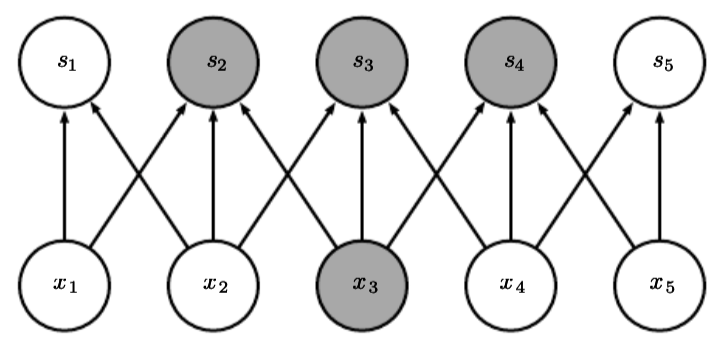
\includegraphics[width=\linewidth]{Images/Chapters/sparsity_1.png}
    \end{minipage}
    \hfill
    \begin{minipage}{0.45\textwidth}
        \centering
        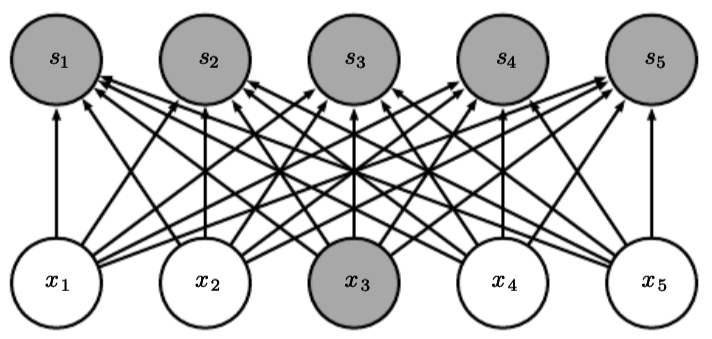
\includegraphics[width=\linewidth]{Images/Chapters/sparsity_2.png}
    \end{minipage}
    \caption{Sparse connectivity: when \textit{s} is formed by convolution (left), and when \textit{s} is formed by matrix multiplication (right).}
    \label{fig:sparsity}
\end{figure}



In a deep convolutional network, stacking multiple convolutional layers allows units in deeper layers to have larger receptive fields, enabling them to capture more abstract and global features by efficiently constructing complex interactions from simple local ones.

\begin{figure}[H]
    \centering
    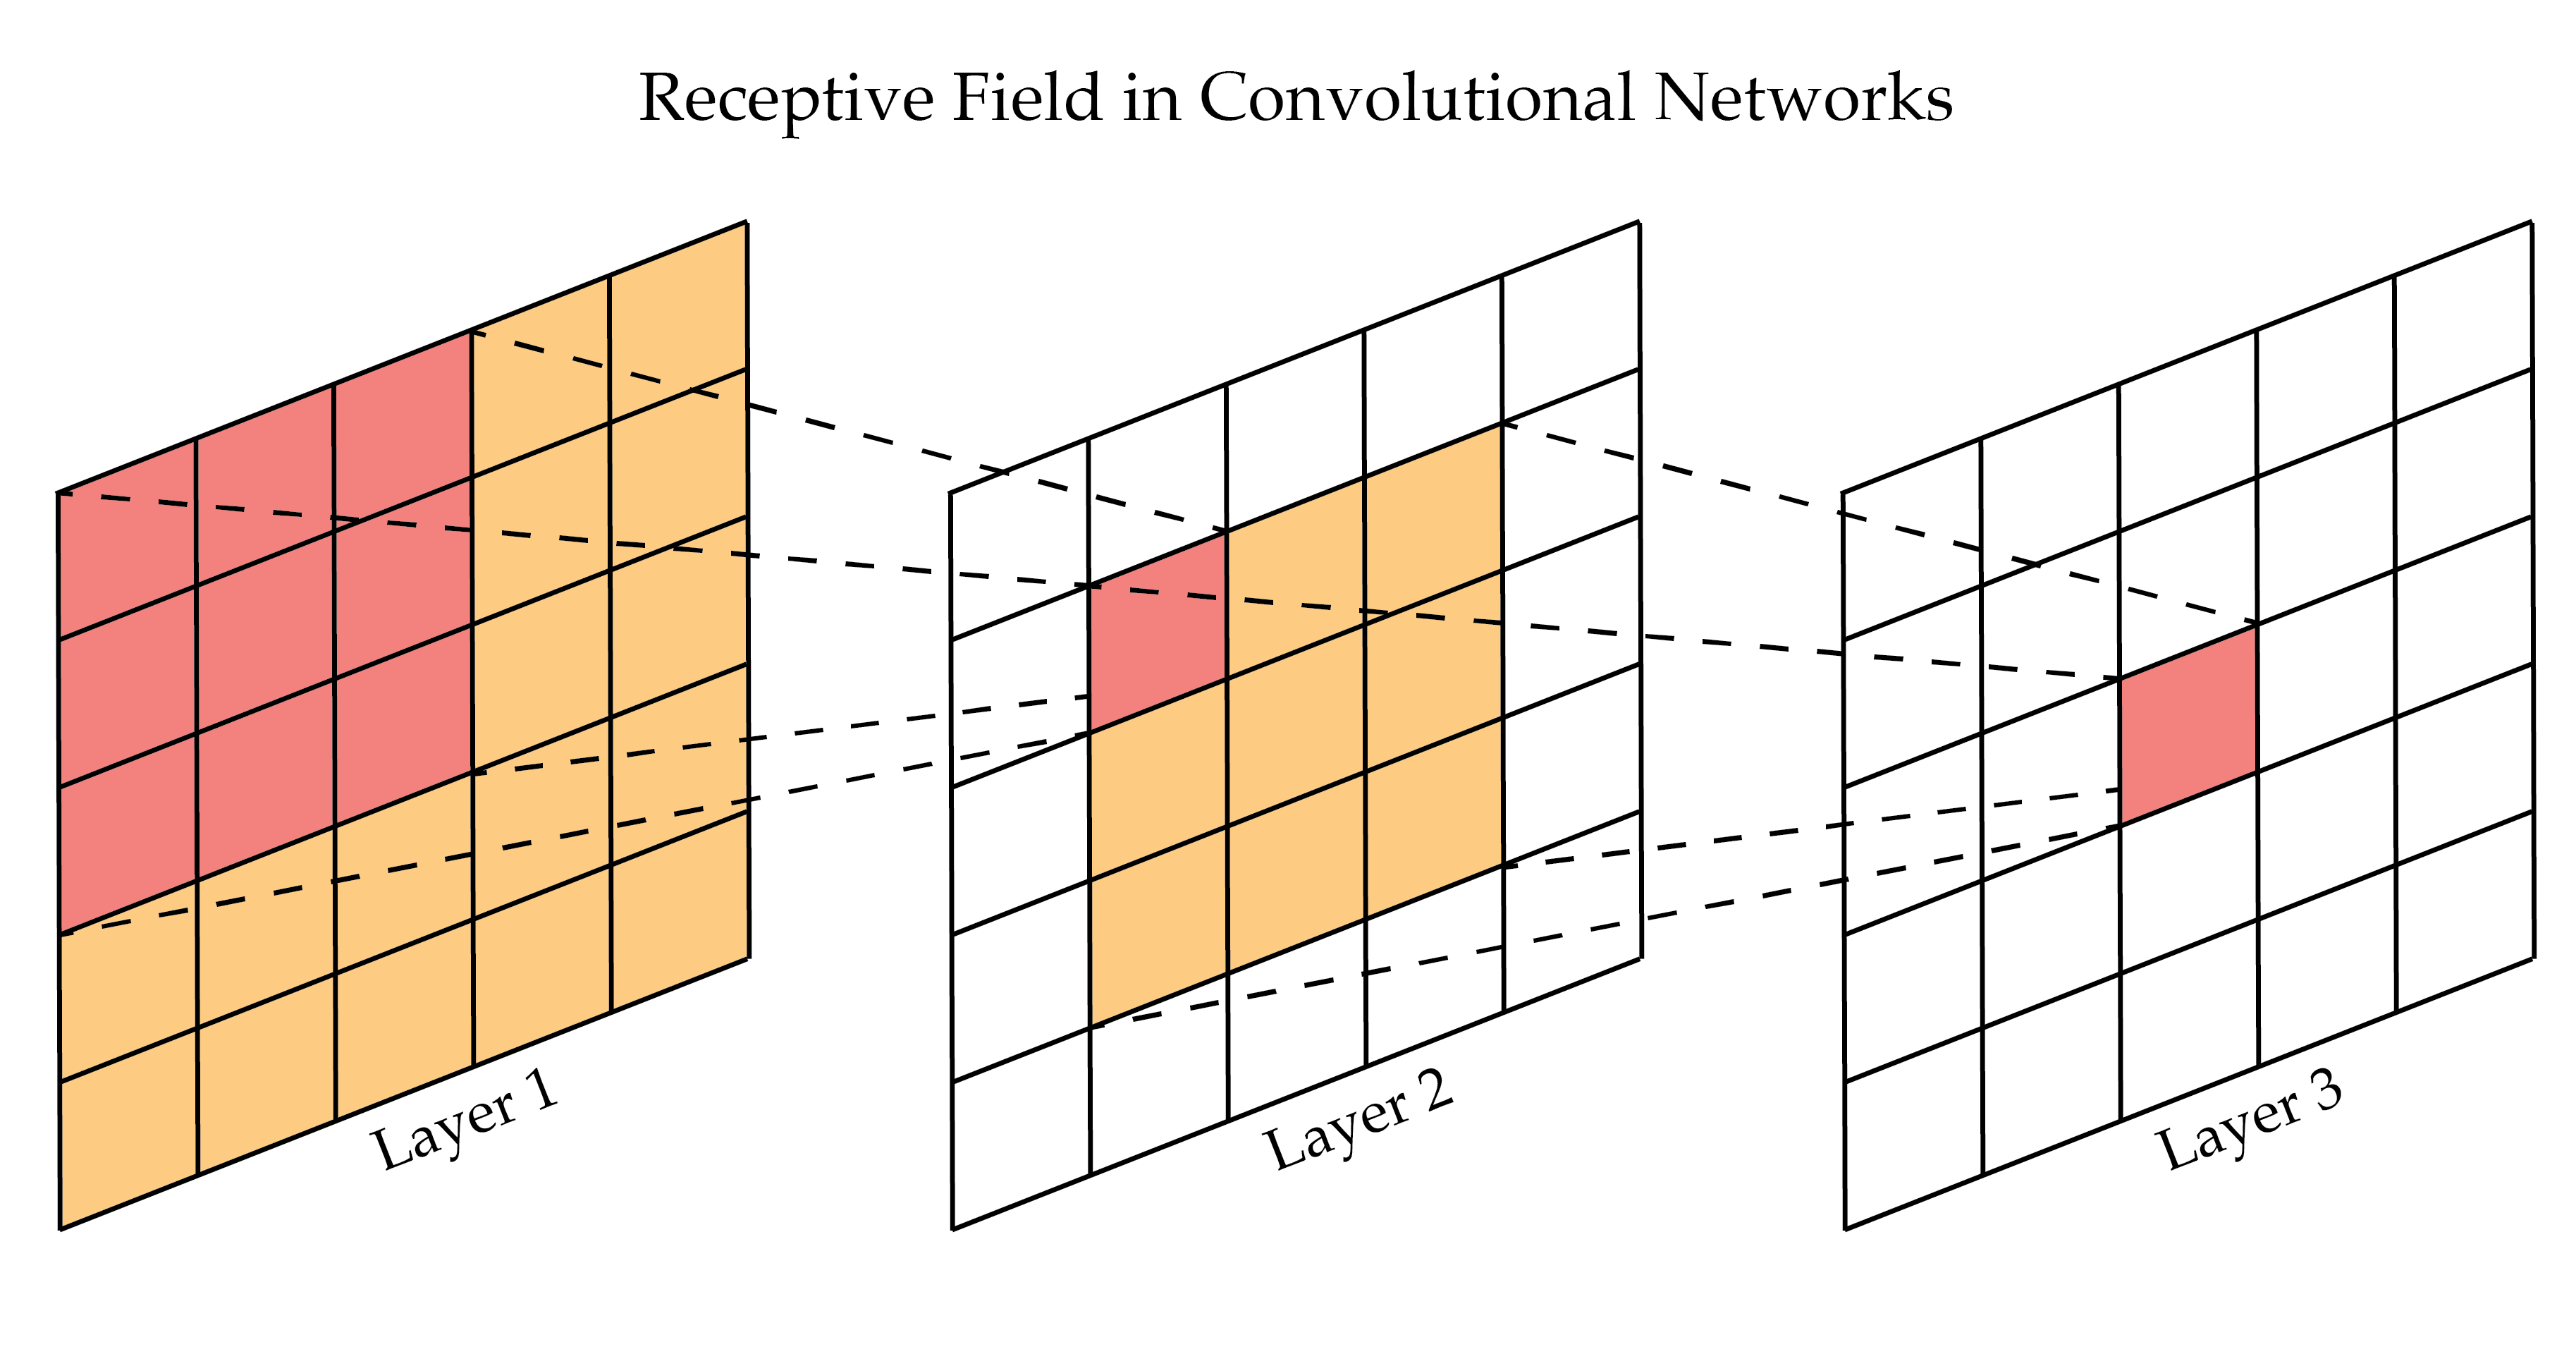
\includegraphics[width=0.5\linewidth]{Images/Chapters/receptive_fields.png}
    \caption{Visualization of growing receptive fields across CNN layers.}
    \label{fig:receptive_fields}
\end{figure}

\section{Parameter sharing}

Another advantage of convolution is that the same kernel is applied across all spatial locations.  
We can say that the network has \textit{tied weights}, because the values of the weight are the same everywhere. This means that instead of learning a separate set of weights for each location, the model learns only one kernel that is reused.  

For example, a kernel that detects vertical edges will detect them anywhere in the image. This does not affect the runtime of forward propagation, still $O(k\times n)$ where $k$ is the kernel size and the input is $m\times n$.

\clearpage

This greatly reduces the number of learnable parameters and improves generalization, since the same features are useful at multiple positions.

\begin{figure}[H]
    \centering
    \begin{minipage}{0.45\textwidth}
        \centering
        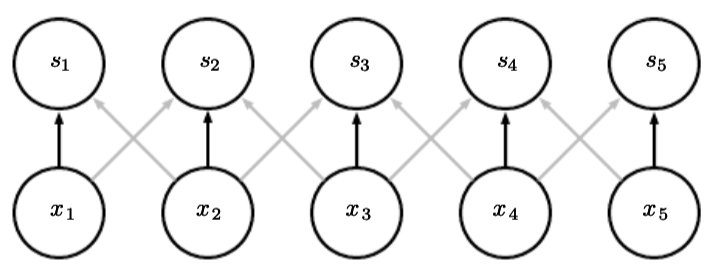
\includegraphics[width=\linewidth]{Images/Chapters/param_sharing2.png}
    \end{minipage}
    \hfill
    \begin{minipage}{0.45\textwidth}
        \centering
        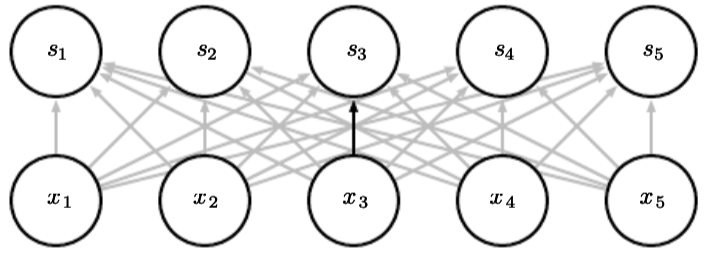
\includegraphics[width=\linewidth]{Images/Chapters/param_sharing1.png}
    \end{minipage}
    \caption{Parameter sharing: because of parameter sharing, the single parameter is used everywhere (left); in the other hand the parameter is used only once (right).}
    \label{fig:param_sharing}
\end{figure}

\section{Equivariance to translation}

The already discussed parameter sharing causes in convolution a property called \textit{equivariance} to translation.  
Formally, a function $f$ is equivariant to an operation $T$ if, applying $T$ to the input and then $f$, gives the same result as applying $f$ first and then $T$ to the output.  

Convolution satisfies this property with respect to translations:  
\[
(K * I)(x + \Delta) = T_{\Delta} \big( (K * I)(x) \big),
\]
where $T_{\Delta}$ denotes a translation by $\Delta$.  

This means that if the input image is shifted, the output feature map shifts in the same way. In images, convolution produces a 2-D feature map where detected patterns shift consistently with the input, enabling parameter sharing across locations. This is useful for features like edges, which appear throughout an image, though in some cases, such as face recognition, different regions may require learning distinct features. 

\chapter{Pooling}

A standard layer in a convolutional network is typically composed of three stages. First, multiple convolutions are applied in parallel to generate linear activations. Next, these activations are passed through a nonlinear activation function, a step sometimes referred to as the \textit{detector stage}. Finally, a \textit{pooling operation} is applied to further transform and condense the output.

\begin{figure}[H]
    \centering
    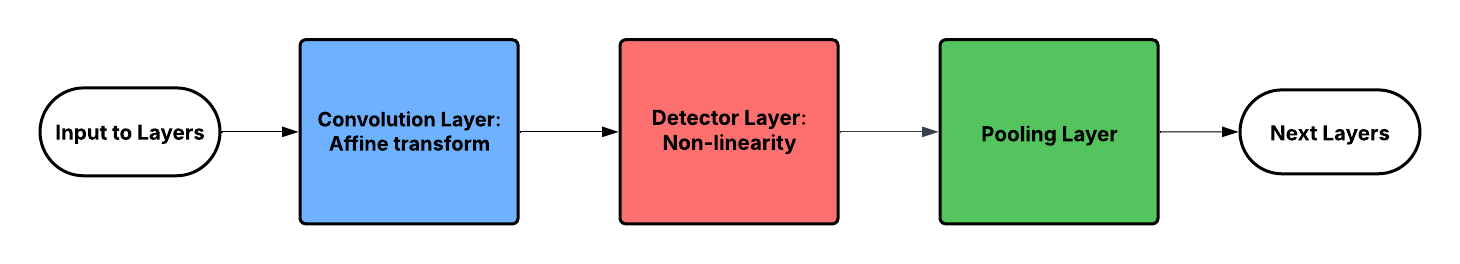
\includegraphics[width=0.7\linewidth]{Images/Chapters/layers.png}
    \caption{Data flow through a typical CNN block.}
    \label{fig:cnn_block_flow}
\end{figure}

Pooling is a subsampling operation that has traditionally played a central role in CNNs.  
Its purpose is to reduce the spatial resolution of feature maps while retaining the most important information. The use of pooling can be viewed as adding an infinitely strong prior that the function the layer learns must be invariant to small translations. When this assumption is correct, it can greatly improve the statistical efficiency of the network \cite{goodfellow2016deep}.
However, when the assumption does not hold, convolution and pooling may actually harm performance. 
Like any prior, these operations are only beneficial when their underlying assumptions are accurate: if a task requires preserving precise spatial information, excessive pooling can increase training error and lead to underfitting. 
For this reason, some architectures apply pooling selectively, on certain channels but not others, to balance the extraction of invariant features with the preservation of fine-grained spatial details.

\section{Definition}

Given an input feature map $X \in \mathbb{R}^{m \times n}$, pooling partitions $X$ into non-overlapping regions and summarizes each region by a statistic.  
The two most common pooling operations are:  

\begin{itemize}
    \item \textbf{Max pooling}, which reports the maximum value within a rectangular \newline neighborhood:
    \begin{equation}
    Y[i,j] = \max_{(p,q) \in \mathcal{R}_{ij}} X[p,q],
    \end{equation}

    \item \textbf{Average pooling}, which computes the mean value:
    \begin{equation}
    Y[i,j] = \frac{1}{|\mathcal{R}_{ij}|} \sum_{(p,q) \in \mathcal{R}_{ij}} X[p,q],
    \end{equation}
\end{itemize}

where $\mathcal{R}_{ij}$ denotes the receptive field corresponding to output element $(i,j)$.  


\section{Motivation and role in CNNs}

The central benefit introduced by pooling lies in the approximately \textbf{invariance to small translations} of the input.

Both max pooling and average pooling summarize local neighbourhoods in a way that makes the representation less sensitive to small shifts in the input.  
This invariance is particularly valuable in visual recognition tasks, when we care more about whether some feature is present than exactly where it is. For example, when recognizing whether an image contains a car, the network does not need to know the exact pixel-level positions of the wheels; it is enough to detect that there are four wheels, with two in the front and two in the back, regardless of small variations in their precise location.

\clearpage

It's also possible, if pooling over the output of separately parametrized convolutions, to make features able to learn \textit{which} transformations to become invariant to.

\begin{figure} [H]
    \centering
    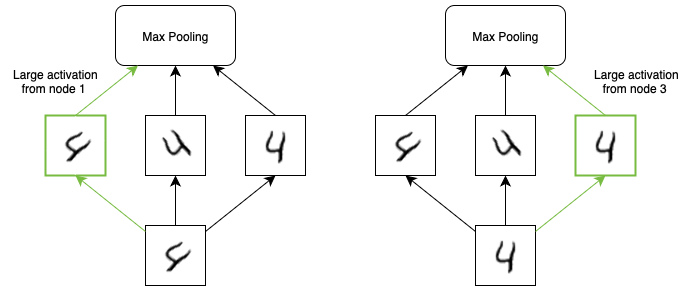
\includegraphics[width=0.7\linewidth]{Images/Chapters/pooling_invariance.png}
    \caption{Example of filters that learn to become invariant to rotation.}
    \label{fig:pooling_invariance}
\end{figure}

Pooling also introduces several important benefits: reduces the spatial resolution of feature maps, which decreases the computational cost of subsequent layers, lowers memory requirements and improves the statistical efficiency of the network by enforcing more compact and robust representations.  

Within the hierarchy of a CNN, pooling therefore plays a key role: early convolutional layers detect local features such as edges, and pooling combines them into progressively more abstract and stable patterns, supporting the network in building higher-level representations \cite{goodfellow2016deep}.


\section{Modern alternatives}
\label{sec:pooling-alternatives}%

While max and average pooling have been widely used, more recent research has explored alternatives that either replace pooling entirely or refine it.  

Springenberg et al., 2015 \cite{springenberg2015allcnn} investigated whether pooling is truly necessary for state of the art performance. They proposed an extremely simple architecture consisting only of convolutional layers, with dimensionality reduction achieved exclusively by \textbf{strided convolutions} (stride of 2).  
Despite the absence of pooling, normalization layers or complex activation functions, this homogeneous architecture was able to achieve competitive, and in some cases state of the art, performance on benchmark datasets such as CIFAR-10, CIFAR-100, ImageNet.   Their findings demonstrated that small convolutional layers with stride can be sufficient to replace traditional pooling operators and raises important questions about the necessity of pooling in CNNs.
 
Traditional pooling operations either discard information (max pooling) or average it uniformly (average pooling), both of which may lead to a loss of useful detail.  
\textbf{SoftPool} (Stergiou et al., 2021 \cite{stergiou2021softpool}) addresses this limitation by computing a weighted average, where the weights are proportional to the magnitude of the activations within each pooling region.  
This mechanism allows more information to be preserved, while still reducing the spatial resolution of the feature maps. Experimental evaluations have shown that SoftPool improves classification accuracy on benchmarks such as ImageNet, CIFAR, and Kinetics, while introducing only minimal computational overhead.  
These results suggest that more informative pooling operators can provide benefits over max and average pooling and highlight the potential of adaptive downsampling methods in modern CNNs.

\chapter{Variants of the Basic Convolution Function}

In the context of neural networks, we do not usually apply the standard convolution operation, as presented in Chapter \labelcref{ch:what-is-conv}. The convolution operation at the core of CNNs admits several useful modifications that expand its flexibility and efficiency.  
The variants of the basic convolution functions can differ slightly in how parameters are shared, how receptive fields are enlarged or how the computation is factorized.  

\section{Strided convolution}

When dealing with images, software implementations usually work in batch mode, so they use as input and output of the convolution some 4-D tensors, with the first index into the different channels, the following two indices into the spatial coordinates of each channel and the fourth axis indexing different examples in the batch. 

Assume we have 4-D kernel tensor $K$ with element $K_{i,j,k,l}$ giving the connection strenght between a unit channel in channel $i$ of the output and a unit in channel $j$ of the input, with an offset of $k$ rows and $l$ columns between the output unit and the input unit. Assume our input consists of observed data $v$ with element $V_{i,j,k}$ giving the value of the input within channel $i$ at row $j$ and column $k$. Assume our output consists of $Z$ with the same format as $V$. If $Z$ is produced by convolving $K$ across $V$ without flipping $K$, then:

\begin{equation}
    Z_{i,j,k}=\sum_{l,m,n}V_{l,j+m-1,k+n-1}K_{i,l,m,n}
\end{equation}

where the summation over $l, m$ and $n$ is over all values for which the tensor indexing operations inside the summation are valid.

In standard convolution, the kernel is applied at every possible location in the input. A simple modification consists of applying the kernel only at locations separated by a fixed step size, known as the \textit{stride}. Formally, for stride $s$, the output of the convolution is defined only at positions spaced $s$ units apart:

\begin{equation}
    Z_{i,j,k}=c(K,V,s)_{i,j,k}=\sum_{l,m,n}[V_{l,(j-1)\times s+m,(k-1)\times s+n}K_{i,l,m,n}]
\end{equation}
 
\clearpage

This reduces the spatial resolution of the output and combines the effects of convolution and subsampling. We already saw that \textit{strided convolution} is often used as an alternative to pooling, section \labelcref{sec:pooling-alternatives}.  

\section{Zero-padding}

Another common variant is related to the ability of \textit{zero-padding}, where the input is padded with zeros around its border before applying convolution, to make it wider. Zero-padding allows control over the size of the output feature maps.  
Without padding, the spatial dimensions shrink after each convolution; with appropriate padding, the output can be kept at the same size as the input.

\begin{figure} [H]
    \centering
    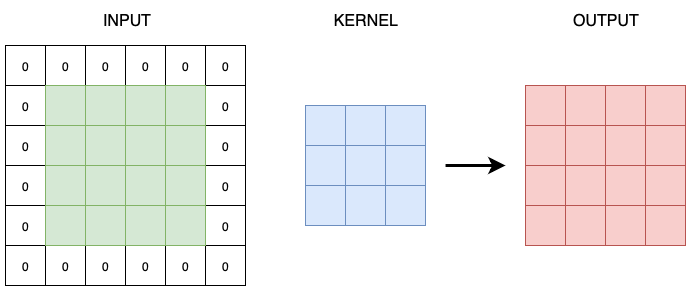
\includegraphics[width=0.7\linewidth]{Images//Chapters/zero_padding.png}
    \caption{Example of zero padding equal to one.}
    \label{fig:zero_padding}
\end{figure}

The most common conventions are: \textbf{valid convolution} in which no padding is applied, so for a one-dimensional input of length $m$ convolved with a kernel of size $k$ the output length is $m - k + 1$; \textbf{same convolution} where padding is chosen so that the output has the same size as the input, i.e.\ $m$; \textbf{full convolution}, here padding is added so that the kernel can be applied at every possible shift, producing an output of size $m + k - 1$.  

\section{Unshared and Tiled Convolution}

In a standard convolutional layer, the same kernel is applied across all spatial locations. This weight sharing greatly reduces the number of parameters.  
However, we can relax this assumption, leading to the concept of \textit{locally connected layers}.  

The most general case is the \textbf{unshared convolution} where each output unit has its own distinct set of weights rather than sharing the same kernel across all positions.

\clearpage

Formally, let $x \in \mathbb{R}^{n}$ be a one-dimensional input and suppose we use windows of size $k$ to produce an output $y \in \mathbb{R}^{m}$.  
In a standard convolution, the same kernel $w \in \mathbb{R}^{k}$ is used at all locations. In the unshared case, each position $i$ has its own kernel $w^{(i)} \in \mathbb{R}^{k}$, yielding:

\begin{equation}
y_i = \sum_{j=1}^{k} w^{(i)}_j \, x_{i+j-1}, \quad i=1,\dots,m.
\end{equation}

This increases the number of parameters from $k$ to $m \times k$, and in higher dimensions from $k^2$ to $m \times n \times k^2$, making the model far less efficient.  
Locally connected layers are useful when we know that each feature should be a function of a small part of space, but there is no reason to think that the same feature should occur across all of space. 

Between the two extremes of full parameter sharing (\textit{standard convolution}) and no sharing (\textit{unshared convolution}), there exists an intermediate approach known as \textbf{tiled convolution}.  
In this variant, weights are shared, but only among a restricted set of positions.  
For example, one might specify a tiling factor $t$, such that every $t$ consecutive locations reuse the same kernel, after which a new set of weights is introduced.  

Formally, let $w^{(1)}, \dots, w^{(t)}$ denote $t$ different kernels.  
At position $i$, the kernel used is determined by $w^{(i \bmod t)}$, i.e.

\begin{equation}
y_i = \sum_{j=1}^{k} w^{(i \bmod T)}_j \, x_{i+j-1}.
\end{equation}

This design relaxes the strong prior of full translation equivariance while still controlling the number of parameters compared to the fully unshared case.  
It allows the model to learn features that vary smoothly across space, without requiring each location to have an entirely independent set of weights.  

Locally connected and tiled convolutional layers exhibit a particular interaction with max pooling: their detector units rely on distinct filters. When these filters capture different transformed versions of the same feature, the subsequent max pooling operation produces units that are invariant to such transformations. (Figure \labelcref{fig:pooling_invariance}).  

\section{Separable convolution}

A kernel can sometimes be factorized into simpler components.  
For example, a 2D convolution with a $k \times k$ kernel can be replaced by two 1D convolutions ($k \times 1$ followed by $1 \times k$).  
This is known as \textit{spatially separable convolution} and it reduces computation when the factorization is exact or a good approximation.  

\clearpage

An important extension is the \textit{depthwise separable convolution}, introduced in MobileNets, 2017 \cite{howard2017mobilenets}.  
This factorizes convolution into two steps:  
\begin{enumerate}
    \item a \textit{depthwise convolution}, where each filter is applied independently to a single input channel;  
    \item a \textit{pointwise convolution}, using $1 \times 1$ kernels to combine information across channels.  
\end{enumerate}
This decomposition greatly reduces the number of parameters and multiplications, enabling efficient CNNs suitable for mobile and embedded devices.

\chapter{Applications of Convolution to Different Data Types}

Convolutional networks are not limited to images.  
The same mathematical operation can be applied to different data types, depending on their structure and dimensionality. In this section we review the most common cases.  

\section{One and Two dimensional data}

The simplest applications of convolution are to one-dimensional and two-dimensional arrays.  
In the one-dimensional case, typical of time series or audio signals, convolutional filters slide along the temporal axis, detecting short-term dependencies, periodicities or characteristic frequency components.  
This makes 1D convolution suitable for speech recognition, time-series forecasting and other tasks where local temporal context is important.  

In the two-dimensional case, characteristic of image data, the input is arranged in a grid of pixels (with additional channels for color).  
Here, convolutional kernels learn to capture local spatial features such as edges, textures and corners.  
By stacking multiple layers, the network progressively builds more complex and abstract representations, forming the foundation of modern computer vision systems.  

\section{Higher-dimensional data: video and volumetric analysis}
\label{sec:3D-CNNs}%

Convolution naturally extends to three or more dimensions.  
A key application is in video understanding, where the input has two spatial dimensions and one temporal dimension.  
In this case, 3D convolutional kernels are used to jointly model motion and appearance, enabling the detection of spatio-temporal patterns such as moving objects, gestures, or human actions.  

\clearpage

Ji et al. \cite{ji2013} proposed one of the first effective 3D CNN architectures for human action recognition.  
Their model performs convolutions over both spatial and temporal dimensions by applying 3D kernels to small cubes of consecutive video frames.  
This design captures motion features that are not accessible to standard 2D CNNs operating on individual frames.

\begin{figure} [H]
    \centering
    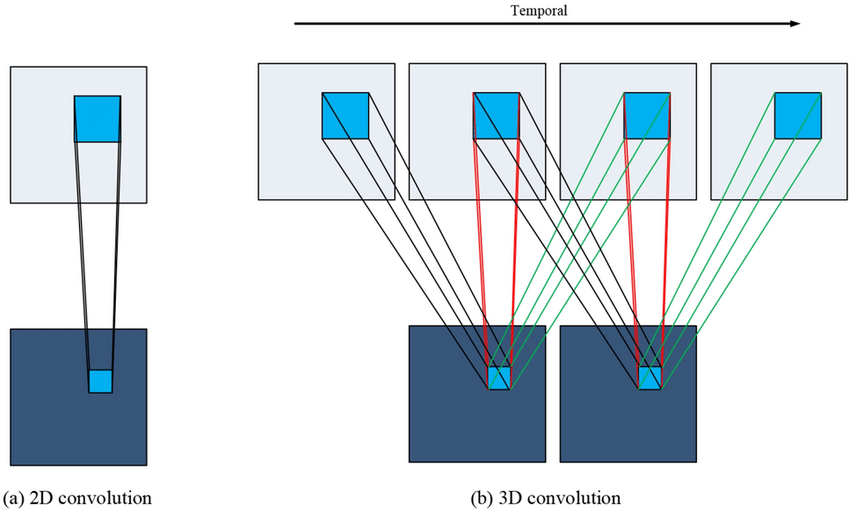
\includegraphics[width=0.7\linewidth]{Images//Chapters/Comparison-between-2D-CNN-and-3D-CNN.png}
    \caption{Comparison between 2D and 3D CNN}
    \label{fig:2Dvs3DCNN}
\end{figure}

Formally, the value at position $(x, y, z)$ on the $j$th feature map in the $i$th layer is given by

\begin{equation}
v^{xyz}_{ij} = \tanh \left( b_{ij} + 
\sum_{m} \sum_{p=0}^{P_i-1} \sum_{q=0}^{Q_i-1} \sum_{r=0}^{R_i-1} 
w^{pqr}_{ijm} \, v_{(i-1)m}^{(x+p)(y+q)(z+r)} \right),
\end{equation}

where $(P,Q,R)$ are the spatial and temporal dimensions of the kernel, $w^{pqr}_{ijm}$ are the kernel weights, and $b_{ij}$ is the bias.  

The proposed architecture was evaluated on large-scale datasets such as TRECVID surveillance videos and the KTH human action dataset. The results showed that 3D CNNs outperform traditional frame-based (2D CNNs) methods and handcrafted spatio-temporal features, particularly in real-world environments with cluttered backgrounds and viewpoint variations. Interestingly, the gains were more significant when the number of positive training examples was limited, highlighting the statistical efficiency of learned spatio-temporal features.

\clearpage

\chapter{Neuroscientific Principles for CNNs}

Convolutional networks are perhaps the greatest success story of biologically inspired artificial intelligence. Though convolutional networks have been guided by many other fields, some of the key design principles of neural networks were drawn from neuroscience \cite{goodfellow2016deep}.  

\section{Receptive fields in the visual cortex}

Hubel and Wiesel \cite{hubel1968} conducted pioneering experiments on the visual cortex of cats and monkeys. They showed that neurons in early visual system responded selectively to specific regions of the visual field. These regions, known as \textit{receptive fields}, cover only a small portion of the visual input. Moreover, many neurons respond preferentially to simple patterns such as oriented edges or bars of light.

In the perspective of deep learning, we can consider a very simplified view of brain function. According to this view, that early visual system identified is called \textbf{V1}, also known as the \textit{primary visual cortex}, located in the back of the head.

This suggested a hierarchical organization: lower-level neurons detect simple visual features, while higher-level neurons combine them to represent more complex structures.  

\section{Translation to convolutional models}

Convolutional networks reproduce several key properties observed in the primary visual cortex. V1 is organized as a spatial map: neurons respond to specific regions of the visual field, preserving the topographic organization of the retina.  
CNNs can capture this property by defining features on two-dimensional maps, where each unit corresponds to a localized region of the input.  

Second, V1 contains many \textbf{simple cells}, whose activity can be approximated as a linear function over a small receptive field.  
The detector units in CNNs are designed to emulate these cells, applying learned linear filters to local regions of the input.  

Finally, V1 includes also \textbf{complex cells} which are insensitive to small shifts in the position of features and sometimes to changes such as lighting conditions. This biological mechanism inspires the use of pooling in CNNs.

\clearpage

It is generally believed that the same basic principles of V1 apply to other areas of the visual system. As far as we are concerned, the main role of these other anatomical regions is just to carry the signal to V1. When viewing an object, information flows from the retina, through a brain region called the \textit{lateral geniculate nucleus } (LGN), to V1, then onward to V2, then V4, then to the last layer, the \textit{inferotemporal cortex} (IT). In our vision, as we move deeper into the brain, a basic strategy of detection followed by pooling is repeated.

This alternation of detection and pooling observed across the multiple areas of the visual system (LGN, V1, V2, V4, IT) is mirrored in the layered structure of CNNs.  
As deeper layers combine the outputs of earlier ones, the network builds progressively more abstract features, similar to how the IT encodes complex objects and shows invariance to many transformations. Empirical studies even demonstrate that CNN activations can predict firing rates in IT and achieve performance comparable to humans on rapid object recognition tasks (DiCarlo, 2013 \cite{dicarlo2013}). 

\section{Limitations of the analogy}

Although CNNs were inspired by the described visual system, there are many important differences. Some of these differences are well established in neuroscience, while others remain open questions, as many aspects of biological vision are not yet fully understood.  

A major difference concerns the input itself. Human vision is not uniformly high resolution: most of the retina provides only coarse information, while a small central region called the \textbf{fovea} captures fine detail.  
To perceive a full scene in high resolution, the brain integrates successive glimpses obtained through rapid eye movements known as \textbf{saccades}. Convolutional networks instead, usually process entire images at full resolution in a single pass. 

Another difference is that the human visual system operates in conjunction with other senses such as hearing and is influenced by factors like mood, attention and prior knowledge. CNNs instead are purely visual systems that lack such multimodal integration. Moreover, the biological visual system does much more than object recognition. It interprets complex scenes, reasons about the relationships between objects, and processes 3-D geometric information necessary for action and navigation.  
Convolutional networks have been applied to some of these tasks, as described in section \labelcref{sec:3D-CNNs}, but such applications are still in their infancy.  

Feedback is another critical distinction: even in early cortical areas such as V1, activity is strongly shaped by top-down signals from higher visual areas. Although feedback connections have been studied in artificial neural networks, they have not yet produced consistent advantages comparable to those observed in biology. Finally, while firing rates in IT resemble the features extracted by deep convolutional layers, the intermediate computations may differ substantially. The brain probably uses more complex activation and pooling mechanisms than simple linear filters.

\clearpage

\chapter{Conclusion and Outlook}

Convolutional Neural Networks have transformed machine learning by combining mathematical structure, computational efficiency and inspiration from neuroscience.  
Through convolution, they exploit local connectivity, weight sharing and translation equivariance, while pooling introduces useful invariances and reduces complexity.  
Variants of the basic convolution function extend their flexibility and modern alternatives to pooling demonstrate the adaptability of these models to evolving needs.  
Applications across one, two and three-dimensional data, highlight the generality of convolution as a tool for representation learning.  
The neuroscientific parallels further reinforce the conceptual foundation of CNNs, even though many differences remain between artificial models and biological vision.

Looking forward, convolutional networks are likely to remain central in deep learning, though their dominance is being challenged by newer architectures such as attention based models and transformers.  
Future directions may involve hybrid models that combine convolution with attention or other mechanisms, better approximations of biological processes such as foveation and feedback and broader applications beyond vision, including multimodal learning and scientific data analysis.  

In summary, CNNs illustrate how mathematical principles, engineering solutions and biological insights can converge into models that not only achieve state of the art performance but also continue to inspire new generations of machine learning research.


%-------------------------------------------------------------------------
%	BIBLIOGRAPHY
%-------------------------------------------------------------------------

\addtocontents{toc}{\vspace{2em}} % Add a gap in the Contents, for aesthetics
\clearpage
\bibliography{Thesis_bibliography} % The references information are stored in the file named "Thesis_bibliography.bib"

\end{document}